% TODO: Check the right use of the 'collection' and 'document' terms.
% TODO: Get a better understanding about the entity's score in the LingPipe.
% TODO: Create a way to disambiguate the new annotation with the old annotation.
% TODO: More explain on the conversion from new annotation to old annotion.
% TODO: The Java application isn't extendable, report this.
% TODO: How to work the query compisition
% TODO: Change `.bind()` with someother.

\chapter{Relazione sui compiti svolti}
\label{cap:relazione}

\section{Strutturazione delle attività}
In questo capitolo verranno descritte in modo dettagliato tutte le varie
attività svolte presso la Wonderflow. Ogni sezione raggruppa le mansioni seguite
per realizzare uno specifico prodotto, in modo da esporre in maniera esaustiva
tutte le scelte, gli sviluppi ed i meccanismi messi in atto per portare a
termine il compito.

È da specificare che questo è frutto di un lavoro a posteriori: le varie azioni
conseguite furono pianificate senza una coesione logica e con una certa
discontinuità temporale. Solo a fine esperienza è stato possibile dedurre il
quadro d'insieme, impossibilitando però la produzione di una pianificazione che
seguisse il prodotto dall'inizio alla fine. Anche le stesse mansioni non hanno
sempre potuto godere di una progettazione allegata per via dello scarso
interesse che l'azienda nutre.

\section{Modulo NER}
\label{sec:ner}
\subsection{Esportatore annotazioni dalle recensioni}
\subsubsection{Requisiti}
Il funzionamento del modulo NER è strettamente legato al glossario, la fonte 
dove pesca le annotazioni. Inizialmente il glossario è vuoto quindi i primi 
risultati riporteranno la completa assenza di supporto da parte del modulo, ma 
man mano che vengano aggiunte nuove annotazioni il sistema d'individuazione 
inizierà a svolgere il suo compito. Tuttavia la qualità del servizio nei primi 
periodi risentirà della scarsità d'annotazioni raccolte, impedendo di ottenere
suggerimenti che siano un'aiuto concreto all'analista.

Per evitare le basse \textit{performance} iniziali, la Wonderflow ha composto
un insieme di recensioni dove erano presenti annotazioni attentamente
controllate dai \textbf{Senior Analyst} la quale potevano offrire una buona base
di partenza per il glossario.

Però il fatto delle annotazioni salvate come attributo della recensione d'origine
poneva grossi problemi. In primo luogo, ogni programma che gestiva solo
annotazioni avrebbe dovuto conoscere lo schema delle recensioni, creando un
accoppiamento indesiderato; secondo, la semplicità di gestione ed uso
dell'archivio verrebbe meno, principalmente per il fatto di non avere una
relazione \textit{uno a molti} tra annotazione e recensioni.

Necessariamente progettare uno schema che ponesse l'accento sulle annotazioni
piuttosto che sulle recensioni diventava indispensabile. Altro elemento
fondamentale era compiere l'estrazione e la conversione delle annotazioni al
nuovo formato progettato.

Queste due richieste sono state tradotte nella creazione di:
\begin{itemize}
\item Un \gls{DAO} per gestire oggetti \textit{MongoDB} conformi al nuovo schema
dell'annotazione
\item Script \textit{Node.js} che esporta, modifica e salva le annotazione dal
vecchio al nuovo formato
\end{itemize}

La realizzazione di un \gls{DAO} segue sia una norma interna, dove ogni
entità di natura persistente all'interno della compagnia richiede la
realizzazione di un archivio e di un \gls{DAO} associato, sia la sua effettiva
praticità d'uso.

\subsubsection{Sviluppo}
Data la dipendenza dello script con il modulo \gls{DAO} associato alle nuove
annotazioni è stato considerato valido partire con lo sviluppo di quest'ultimo.

La Wonderflow raggruppa i propri \gls{DAO} in un pacchetto \textit{npm} chiamato
``\textit{models}'' in modo che, ogni qualvolta è richiesto l'accesso al
database, sia sufficiente includerlo nel proprio progetto e importare il
\gls{DAO} desiderato. La parte relativa al progetto è illustrata in figura
\ref{fig:dao_annotation}.

\begin{figure}[H]
\begin{center}
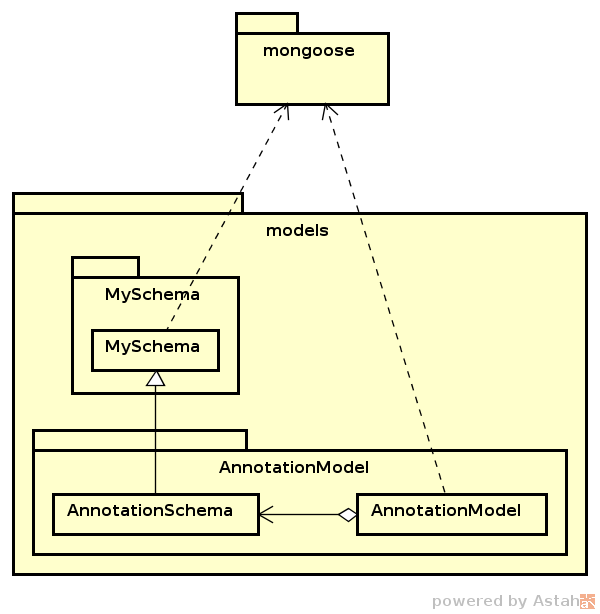
\includegraphics[height=9cm]{dao_annotation}
\caption{
Rappresentazione DAO per le annotazioni nel pacchetto ``\textit{models}''
}
\label{fig:dao_annotation}
\end{center}
\end{figure}

Il package \textit{mongoose} rappresenta il pacchetto \textit{npm} con il quale
vengono implementati i \gls{DAO}. Vi sono due elementi elementi in
\textit{mongoose}: lo \textbf{schema} ed il \textbf{modello}.

Il primo è ciò che rende questo pacchetto molto versatile alla modellazione dei
dati di un'applicazione. Attraverso la definizione di un oggetto in JavaScript, 
è possibile definire di quali \textbf{attributi} il dato da modellare è composto
e quali metodi il \gls{DAO} ha per interfacciarsi con esso. Nel caso in specie,
``\textit{AnnotationSchema}'' definisce come ``annotazione'' un oggetto conforme
al seguente schema:
\begin{center}
\begin{lstlisting}[
  frame=single,
  caption=Schema entità 'annotazione',
  label=valid_annotation]
{
    "uid": "String",
    "name": "String",
    "text": "String",
    "syn": "String",
    "sentiment": 0 | 1,
    "category": "String",
    "status": "String"
    "reviews": [{
       "id": "String",
       "start": "Number",
       "offset": "Number",
       "origin": "pros" | "cons" | "free-text",
       "version": "String"
    }]
}
\end{lstlisting}
\end{center}

mentre il \gls{DAO} eredita i metodi \textit{CRUD (create, read, update,
delete)}\footnote{Per una maggior trattazione si veda
\url{http://coursework.vschool.io/mongoose-crud/}}, implementati dal
``\textit{model}'' base di \textit{mongoose}, ed il metodo per effettuare la
connessione al database da ``\textit{MySchema}''. Inoltre aggiunge un
ulteriore metodo di classe: ``\textit{insertOrMerge}'', di cui se ne 
approfondirà in seguito.

Come si può notare il nuovo schema dell'annotazione è molto simile a quello
risultante dal processo d'analisi, discusso nella sezione
\ref{subsec:processo_recensioni_annotazioni}, ma vi sono alcune differenze che
risolvono egregiamente tutte le problematiche riscontrate:
\begin{itemize}
\item L'annotazione non è più un attributo ma copre il ruolo d'oggetto unico
\item I riferimenti alla recensione in cui appare l'annotazione vengono salvati
nel campo ``\textit{reviews}''
\item Aggiunta attributo ``\textit{status}''
\end{itemize}

Con la prima modifica si rimuove l'accoppiamento indesiderato con la recensione.
Ora un qualsiasi programma che avesse esclusivamente bisogno delle annotazioni
non è vincolato a conoscere la struttura delle recensioni.

Con la seconda modifica invece si gira la relazione \textit{uno a molti} tra
la recensione e l'annotazione, ottenendo che nell'annotazione si mantengono i
riferimenti alle recensioni in cui appare. La gestione dei riferimenti è
compito del \textit{insertOrMerge} citato sopra. La sua funzione è di o inserire
la nuova annotazione se non è già presente o di agganciare i suoi riferimenti 
alle recensioni non ancora presenti nell'attributo ``\textit{reviews}'' di 
quella presente, mantenendo cosi la relazione desiderata.

Infine ``\textit{status}'' viene usato per identificare in quale stato si trova
l'annotazione: \textit{new, archived} o \textit{approved}. Solo le annotazioni
\textit{approved} fanno parte di un glossario.

L'ultimo aspetto da chiarire è il \textbf{modello} di \textit{mongoose},
implementato dalla classe ``AnnotationModel''. Il modello, attraverso lo schema,
funge da costruttore per oggetti legati ad un documento \textit{MongoDB} e
provvisti di tutti i metodi per interfacciarsi. In breve, il modello è il
costruttore dei \gls{DAO}. Nel caso di ``AnnotationModel'' i \gls{DAO}
costruiti sono inerenti alle annotazioni e legati alla collezione
``\textit{Annotation}''.

Una volta completata la parte per accedere e manipolare documenti relativi
alla nuova struttura dell'annotazione, si è prodotto lo \gls{script} per
estrarre le annotazioni già presenti nell'archivio aziendale. Il riassunto del
processo è illustrato in figura \ref{fig:extractor_annotation}.

\begin{figure}[H]
\begin{center}
\includegraphics[height=6cm]{extractor_annotation}
\caption{
Rappresentazione processo d'estrazione e trasformazione delle annotazioni
}
\label{fig:extractor_annotation}
\end{center}
\end{figure}

Lo script è organizzato sottoforma di \gls{pipeline} sfruttando l'interfaccia
``\textit{stream}'' di \textit{Node.js} e la libreria \textit{through2}. La
\gls{pipeline} è composta da tre elementi:
\begin{itemize}
\item ReaderData - legge le recensioni dentro l'archivio e crea lo
\textit{stream}
\item AnnotationExtractor - estrae e applica le debite trasformazioni alle
annotazioni
\item AnnotationWriter - scrive le annotazioni nell'archivio
\end{itemize}

Il ``ReaderData'' usa il \gls{DAO} adibito alle recensioni per leggerle tutte
e generare uno ``\textit{stream}'' con il quale inviarle, di volta in volta,
all'``AnnotationExtractor'' tramite il metodo \textit{.pipe()}.

Il metodo permette la comunicazione tra le unità consecutive della
\textit{pipeline} attraverso la generazione d'eventi il cui contenuto
trasportato è il risultato dell'unita precedente. Nel caso tra ``ReaderData'' e
``AnnotationExtractor'' il contenuto è la recensione estratta, mentre tra
``AnnotrationExtractor'' e ``AnnotationWriter'' è l'annotazione modificata
conforme allo schema \ref{valid_annotation}.

Quando ``AnnotationExtractor'' riceve la recensione applica l'algoritmo di
trasformazione illustrato nel diagramma d'attività
\ref{fig:extractor_annotation}. La recensione in input immagazzina le
annotazioni nell'attributo ``\textit{feature2sentiment}''. Tutte le recensioni
con la versione diversa da ``v2'' vengono immediatamente scartate, in modo da
non complicare l'algoritmo d'estrazione. Il corpo centrale del diagramma ha lo
scopo di ribaltare la relazione tra recensione ed annotazione. Gli attributi:
\textit{version, start, offset e origin} sono dipendenti dalla recensione in
cui l'annotazione era stata individuata; perciò vengono inglobati in un unico
oggetto, identificato con l'id della recensione e inserito nell'attributo
``\textit{reviews}'' dell'annotazione. Una volta terminate tutte le annotazioni,
il risultato finale viene trasmetto all'unità successiva.

\begin{figure}[H]
\begin{center}
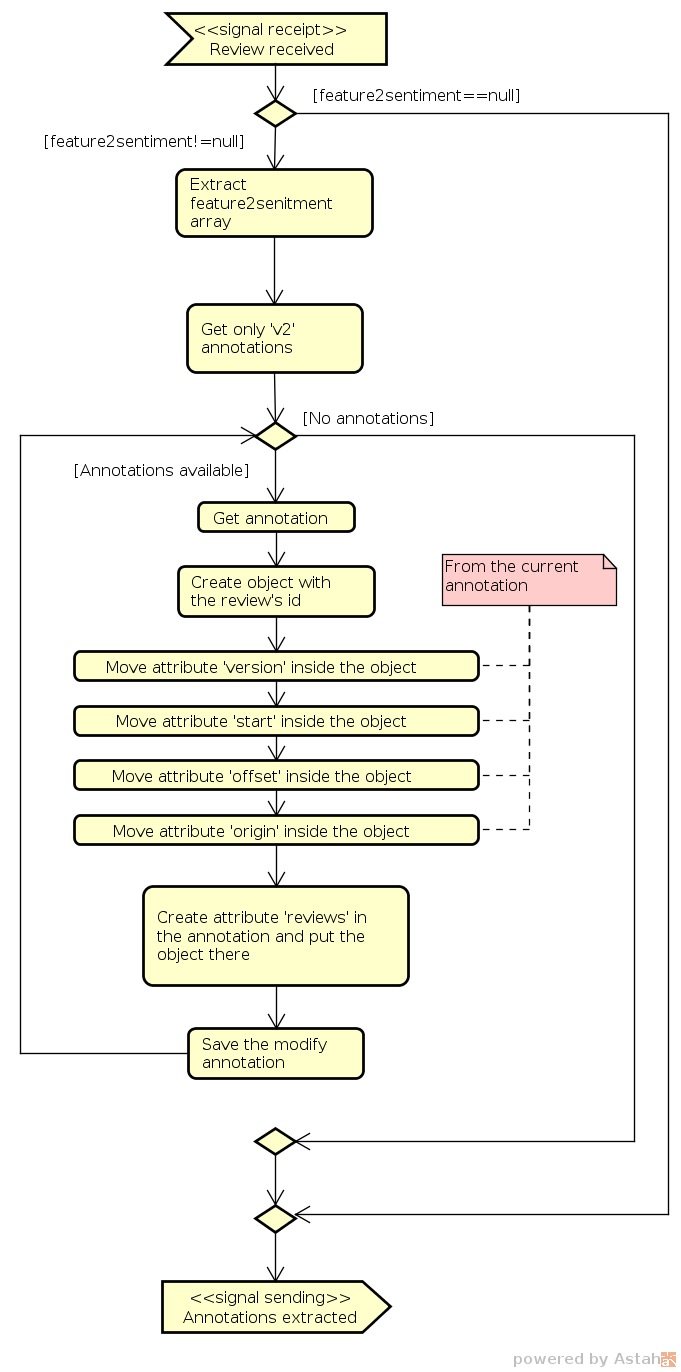
\includegraphics[height=15cm]{extraction_activity}
\caption{
Diagramma d'attività trasformazione annotazioni
}
\label{fig:extraction_activity}
\end{center}
\end{figure}

``AnnotationWriter'' per salvare le annotazioni ricevute nel database, invoca il
metodo \textit{.insertOrMerge()} del \gls{DAO} discusso precedente. In tal modo,
l'unità di scrittura, non dovrà preoccuparsi di come venga mantenuta
la relazione tra annotazioni e recensioni cosi da non violare il
\textit{Single Responsability Principle}.

\subsubsection{Test}
I test svolti nel \gls{DAO} hanno riguardato:
\begin{itemize}
\item L'effettivo salvataggio dell'annotazione
\item La gestione dell'aggiunta della recensione ad un'annotazione che era già
presente nella collezione
\item Controllo che l'aggiunta avvenga solo nel caso di annotazioni uguali.
\end{itemize}

Invece per lo \gls{script} d'estrazione e conversione delle annotazioni è stato
controllato solo se, dato in input un'insieme di recensioni corrette, il
programma terminasse senza alcun errore.

\subsection{Applicazione Java per riconoscere le annotazioni}
\subsubsection{Requisiti}
Il riconoscimento delle annotazioni doveva essere affidato ad un applicazione
Java in modo da usare la libreria \textit{LingPipe} per garantire una certa
efficienza nel portare a termine il compito. Il compito era estendere
un'applicazione Java già esistente, inserendovi le opportune classi per fargli
svolgere il riconoscimento delle annotazioni all'interno di recensioni. In modo
da consentire una rapida integrazione con l'editor messo a disposizione agli
analisti, il formato dell'annotazione doveva essere il medesimo di quello
seguito dall'editor e doveva essere specificata l'origine dal modulo \gls{NER}.

Se rispettati questi requisiti, il modulo \gls{NER} si sarebbe integrato nel
sistema complessivo della Wonderflow senza provvedere ad eventuali adattamenti
sia al sistema sia al modulo stesso.

\subsubsection{Sviluppo}
Non si può negare la vastità di tecniche d'analisi del testo che la libreria
\textit{LingPipe} mette a disposizione. Correzione ortografica, identificazione
della lingua, disambiguazione del significato e analista sentimentale sono solo
alcuni dei possibili problemi che si possono affrontare tramite questa libreria
in ambiente Java. Un'altro possibile è proprio la
\textit{Named Entity Recognition}, l'obiettivo del modulo. Attraverso la
documentazione di \textit{LingPipe} i passi per la creazione di un modulo
\gls{NER} sono risultati molto chiari.

Il sistema di riconoscimento funziona attraverso l'adozione di uno o più metodi
d'individuazione di parole: espressioni regolari, dizionari o modelli
statistici sono quelli citati. In base al metodo scelto si va ad estendere
quella che è la classe usata da \textit{LingPipe} per annotare il testo: il
\textbf{chunk}. Il \textit{chunk} fornisce un punto d'incontro per tutti i vari
metodi, consentendone un uso simultaneo. Nel progetto di stage non è
stata utilizzata questa proprietà, limitandosi all'uso esclusivo del
\textbf{dizionario}. La scelta è stata compiuta in base al sistema delle
annotazioni precedentemente realizzato, risultando molto semplice adattare i
documenti delle annotazioni in entità per il dizionario. Per sistemi \gls{NER}
\textit{LingPipe} espone l'uso di due tipi di dizionari: quello esatto e quello
approssimato. Nel prima caso, le parole associate a menzioni vengono
riconosciute se coincidono alla forma di com'è stata specificata nel dizionario;
nel secondo, tramite il concetto di \textit{distanza}\footnote{Un esempio è la
\textit{distanza di Levenshtein}} tra due parole, si possono ottenere i
riscontri che si avvicinano, anche non combaciando, alle entità del dizionario.

Come prima versione si è scelto di adottare un dizionario esatto per la sua
facilità d'implementazione e per i discreti risultati che si ottengono, già
verificati dall'azienda.

Parlando delle entità da definire nel dizionario, queste sono coppie di valori
\textit{frase-tipo} seguendo la definizione di \textit{Named entity}. Esse
vengono generate a partire dalle nuove annotazioni la quale, attraverso un
processo di codifica, si forma la coppia richiesta. Ogni qualvolta venga trovata
la frase dell'entità nel testo verrà formato un \textit{chunk} contenente:
la frase stessa, il tipo associato, la posizione di partenza e fine nel testo ed
il punteggio associato all'entità. Per le annotazioni, il tipo non è altro che
la compressione delle informazioni non presenti nel \textit{chunk} al fine di
costruire le annotazioni valide per l'editor. La compressione viene eseguita
ottenendo i campi \textit{uid, category, text, sentiment} e generata la stringa
formata dai rispettivi valori separati dalla guardia ``\$\$\$''. Attraverso il
processo di decodifica del tipo ed i gli altri dati forniti dal \textit{chunk}
si è in grado di costruire un'annotazione che segua lo schema
\ref{snippet_annotation_review} associando:

\begin{enumerate}
\item \textit{category, uid, text} e \textit{sentiment} i valori estratti dal
tipo
\item \textit{name} e \textit{syn} è la frase dell'annotazione
\item \textit{offset} e \textit{start} sono inizializzati attraverso il
\textit{chunk}: il primo sottraendo la posizione di fine \textit{match} con la
posizione d'inizio e l'ultimo assegnandoli la posizione d'inizio
\item \textit{version} viene fissato a ``v2''
\item \textit{origin} è scelta in base al corpo della recensione 
(\textit{free-text, pros, cons})
\item \textit{status} è inizializzato con il valore ``new''
\end{enumerate}

Come richiesto nei requisiti, l'annotazione risultante possiede l'attributo
\textit{createdBy} inizializzato con il nome della classe che si occupa di
usare i metodi \textit{LingPipe} per eseguire \gls{NER} e di formare
l'annotazione richiesta.

La progettazione dell'applicazione è illustrata in figura
\ref{fig:tag_recognizer}.

``\textit{SentimentMemoryTagRecognizer}'' è la classe che prende le recensioni,
``\textit{TextReviewForAnalytics}'', e genera la lista delle annotazioni,
``\textit{Annotation}'', trovate usando \textit{LingPipe}. Il metodo
\textit{.findTagsInText()} è l'effettivo metodo che riconosce le annotazioni nel
testo e genera la lista dei risultati. Essendo che una recensione può essere
divisa in tre parti: testo libero, aspetti positivi e negativi;
\textit{.findTagsInReview()} invoca \textit{.findTagsInText()} e nelle
annotazioni risultate riporta la provenienza.

L'operazione di compressione e decompressione viene svolta da
``\textit{SentimentMemoryAnnotationEncoder}'' che espone i metodi necessari per
effettuare sia la codifica, \textit{.encode()}, sia la codifica,
\textit{.decode()}.

Infine, ``\textit{SentimentMemoryTagRecognizerFactory}'' è una versione del
pattern \textit{Factory Method} dove tutta la logica e complessità
dell'algoritmo di costruzione di un oggetto vengono spostate in un'altra entità
che se ne fa carico. Nel caso attuale, nel \textit{factory} è racchiusa la
costruzione del dizionario, necessario alla costruzione di
``\textit{SentimentMemoryTagRecognizer}'' in modo da applicare la ricerca delle
annotazioni. Trammite l'uso del pattern si ambisce al
\gls{separation_of_concerns}, separando come il dizionario viene creato, svolto
dal ``\textit{SentimentMemoryTagRecognizerFactory}'', e il come viene usato,
definito in ``\textit{SentimentMemoryTagRecognizer}''.

\begin{figure}[H]
\begin{center}
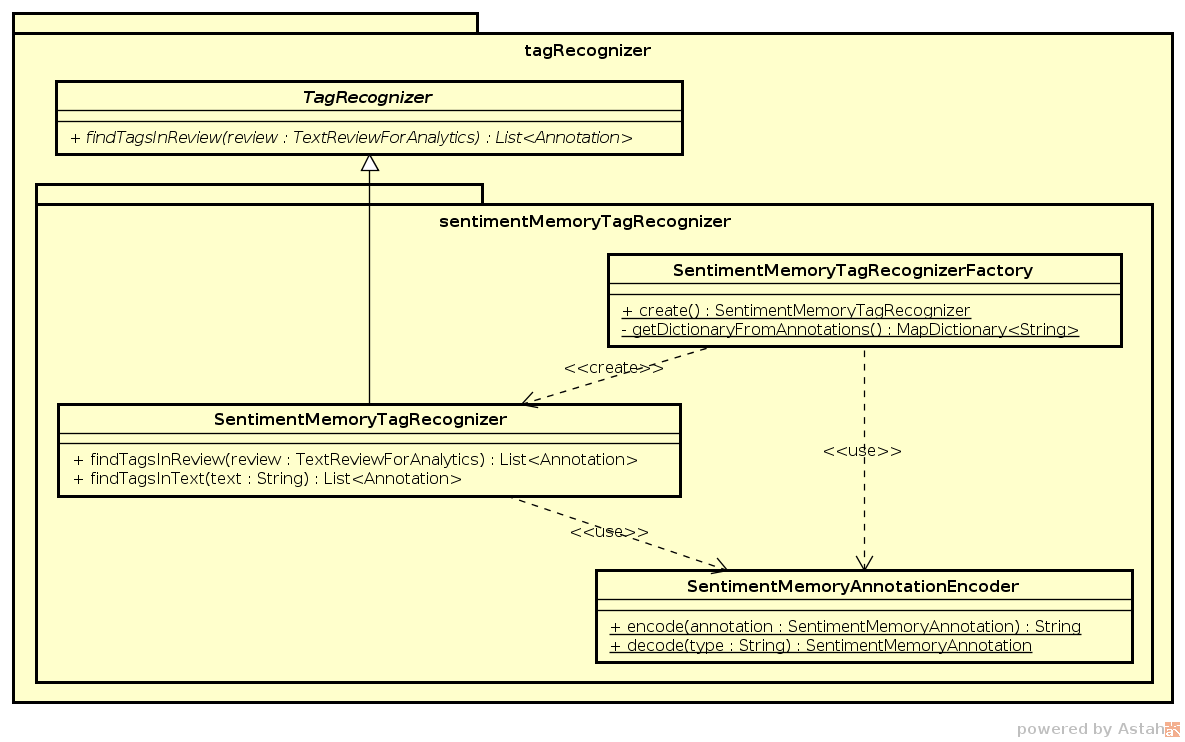
\includegraphics[height=7cm]{tag_recognizer}
\caption{
Diagramma delle classi per il modulo NER
}
\label{fig:tag_recognizer}
\end{center}
\end{figure}

Come era successo nello \gls{script} d'estrazione delle annotazioni, anche qui
si andavano a gestire entità persistenti nell'ecosistema dell'azienda e perciò
si sono implementanti modelli e \gls{DAO} per rappresentarli e gestirli. Le
entità coinvolte nel modulo erano tre: annotazioni del glossario, annotazioni
dell'editor e recensioni. Le ultime due avevano già le classi pronti all'uso,
mentre per il primo è stato necessario realizzarle.

\begin{figure}[H]
\begin{center}
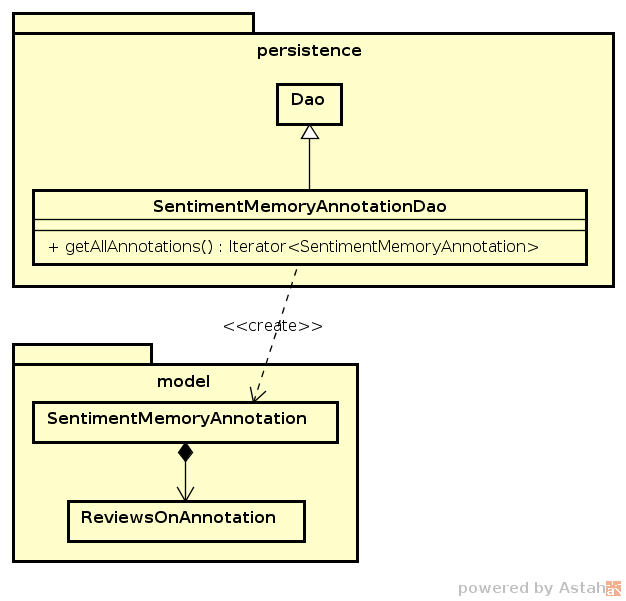
\includegraphics[height=6cm]{model_dao_annotation}
\caption{
Diagramma delle classi per il modello ed il DAO delle annotazioni
}
\label{fig:model_dao_annotation}
\end{center}
\end{figure}

Per implementarle entrambi si è usato la libreria Java \textit{Morphia}, driver
per gestire i documenti di \textit{MongoDB}. Oltre all'accesso effettivo al
database, necessario per realizzare il \gls{DAO}, \textit{Morphia} estende il
sistema delle \textit{annotazioni Java} per mappare classi in documenti in modo
da poterli gestire. 

Riguardo alle classi create, ``\textit{SentimentMemoryAnnotationDao}'' possiede
il metodo per ottenere tutte le annotazioni del glossario, cosi da poterle
caricare nel dizionario di \textit{LingPipe}; mentre
``\textit{SentimentMemoryAnnotation}'' implementa \textit{getter e setter} per
gli attributi presenti in un'annotazione.

L'esecuzione del modulo è a carico di un \textit{runner}, il quale 
altro non è che una implementazione del \textit{Façade pattern} dove ogni 
metodo sono le operazioni eseguibili dall'applicazione Java, compreso il 
sistema di riconoscimento delle annotazioni. L'approccio potrebbe degenerare
nella formazione di una \textit{fat interface} ma l'azienda non prevede 
l'aggiunta di molte funzionalità al programma. A mio avviso l'uso del
\textit{Command Patter} avrebbe garantito una maggiore estensibilità, senza
introdurre difficoltà progettuali. Il comportamento del \textit{runner} viene
gestito tramite file di configurazione in formato \gls{JSON} dove si vanno a
specifiare:
\begin{itemize}
\item Nome dell'azione da eseguire, attributo \textit{run}
\item Url del database \textit{MongoDB} da utilizzare, attributo
\textit{database}
\end{itemize}

In questa fase non era richiesta l'implementazione del metodo d'avvio del modulo
\gls{NER} perchè sarebbe stata affrontata durante la fase d'integrazione con
l'editor usato dagli analisti.

\subsubsection{Test}
I test sono stati eseguiti sui metodi di
``\textit{SentimentMemoryTagRecognizerFactory}'' e
``\textit{SentimentMemoryTagRecognizer}''.

\paragraph{SentimentMemoryTagRecognizerFactory.create()}
Il test consisteva nella creazione di un'istanza di
``\textit{SentimentMemoryTagRecognizer}'' con associato un dizionario di
annotazioni formato da due elementi caricati precedentemente da una collezione
\textit{MongoDB} in locale. Con \textit{.getDictionary()} di
``\textit{SentimentMemoryTagRecognizer}'' si andava a recuperare il dizionario
per estrarre il numero degli elementi contenuti. Il test passava se la
cardinalità del dizionario coincideva con il numero di annotazioni caricate.

\paragraph{SentimentMemoryTagRecognizer.findTagsInReview()}
Il test iniziava con la compisizione di una recensione modello con le due
caratteristiche
\begin{itemize}
\item Erano definite le tre parti di una recensione: \textit{pros, cons} e
\textit{free-text}
\item Tutte le annotazioni del dizionario erano presenti nelle tre parti.
\end{itemize}
successivamente si eseguiva il metodo \textit{.findTagsInReview()} per ottenere
la lista delle annotazioni. Il test passava quando la lista aveva tanti elementi
quante le annotazioni attese e ogni annotazioni possedeva il campo
\textit{sentiment} e \textit{origin} inizializzato con:
\begin{enumerate}
\item (0, ``cons'') - se l'annotazione provenisse dai \textit{cons} della
recensione
\item (1, ``pros'') - se l'annotazione provenisse dai \textit{pros} della
recensione
\item origin uguale a ``free-text'' se l'annotazione provenisse dal
\textit{free-text} della recensione, l'attributo \textit{sentiment} non veniva
controllato
\end{enumerate}

\paragraph{SentimentMemoryTagRecognizer.findTagInText()}
A differenza del test sopra, qui si assicurava che le annotazioni trovate
siano complete e ogni attributo abbia il giusto valore. Per eseguirlo si è
usata direttamente un testo piano, salvato in una stringa, ed eseguito il metodo
\textit{.findTagInTextTest()} per ottenere la lista di annotazioni presenti.

L'analisi degli attributi veniva eseguita solo su quella in testa alla lista.

\subsection{Integrazione con il tool esistente, l'editor di annotazioni}
\subsubsection{Requisiti}
L'unico requisito espresso è che le annotazioni create attraverso l'applicazione
Java fossero salvate nelle recensioni che si sarebbero andate ad analizzare.
Più precisamente, le annotazioni sarebbero state aggiunte all'array associato
all'attributo \textit{feature2sentiment} della recensione.

\subsubsection{Sviluppo}
Come spiegato nella sezione precedente, per dare la possibilità di avviare il
modulo era sufficiente aggiungere un metodo al \textit{runner} dell'applicazione
che eseguisse l'analisi delle recensioni e salvasse i risultati nel database.

Il metodo è riassunto nell'immagine del diagramma di sequenza
\ref{fig:runner_sequence}.

\begin{figure}[t]
\begin{center}
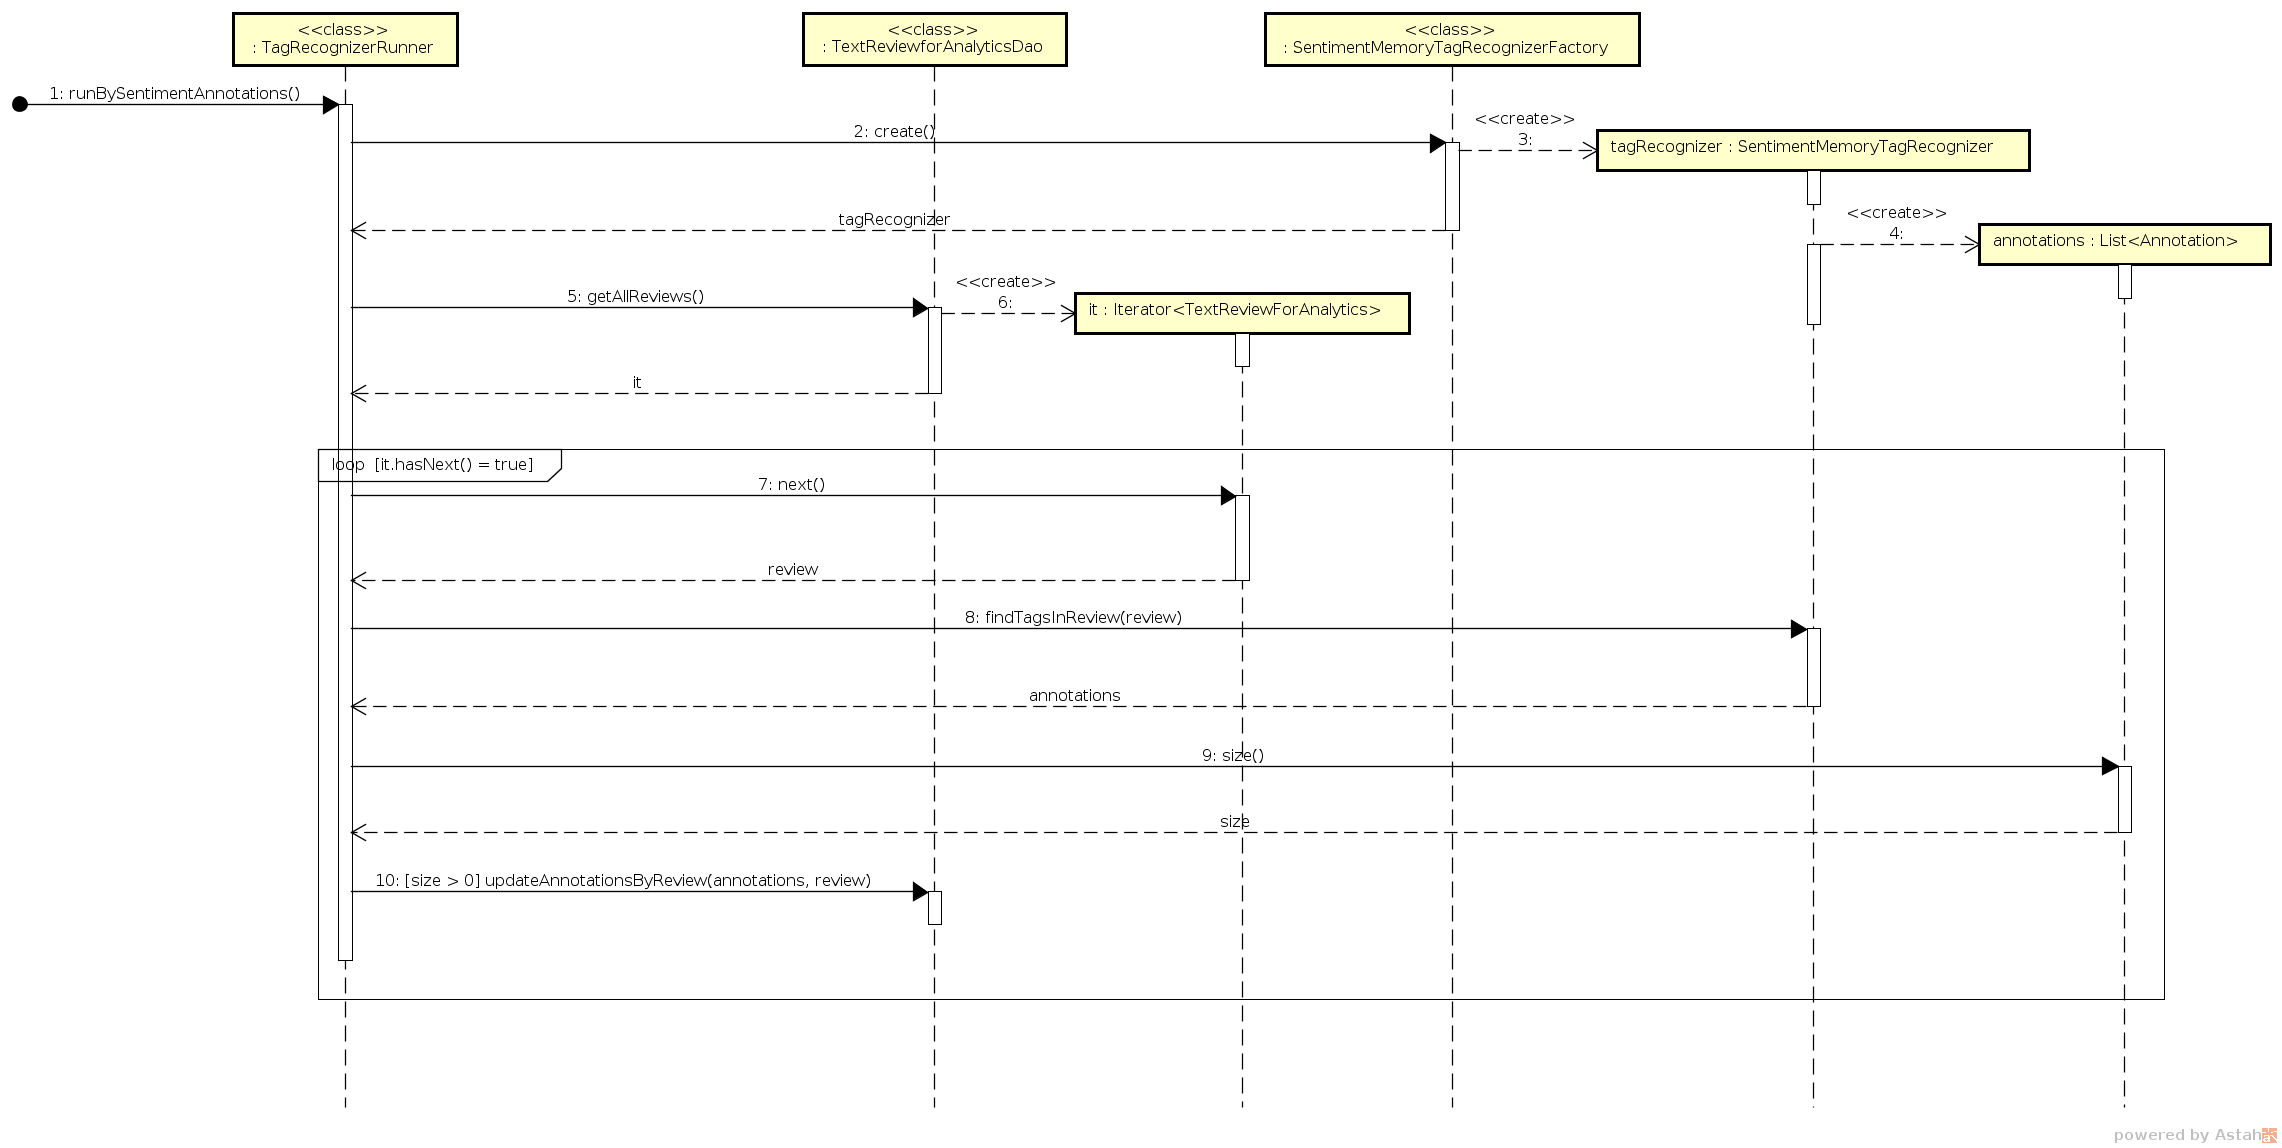
\includegraphics[height=8cm]{runner_sequence}
\caption{
Diagramma di sequenza per il metodo di esecuzione del modulo NER
}
\label{fig:runner_sequence}
\end{center}
\end{figure}

Una volta sviluppato le altre operazioni riguardavano solo il file di
configurazione del modulo \gls{NER}. Nel campo \textit{database} è stato
riportato l'indirizzo del database aziendale dove sono tenute le collezioni
delle recensioni e del glossario; invece in \textit{run} si è trascritto il nome
della \textit{subroutine} di riconoscimento delle annotazioni.

E' da specificare che il processo d'analisi automatica richiede l'intervento
periodico di un operatore umano, in quanto l'azienda non è in possesso di alcun
sistema d'automazione.

\subsubsection{Test}
Non sono stati sviluppati test in quanto le parti che vanno a comporlo sono
state già collaudate e non si è visto la necessità di crearli visto la
dimensione ridotta della funzione. Per quanto riguarda il \textit{tool} usato
dagli analisti, neanche li vi è stato nessuna creazione di test in quanto il
modulo per l'editor era già stata creato e collaudato precedentemente
dall'azienda.
%\subsubsection{Script di misurazione qualità}
%

\section{Moderazione del glossario}
\label{sec:glossary}
\subsection{Comunicazione con il backend}
\subsubsection{Requisiti}
Prima di partire con lo sviluppo dell'interfaccia per moderare il glossario, era
necessario creare un collegamento tra l'applicazione web ed i dati archiviati
nel database.

Come spiegato le applicazioni seguono il modello del
\gls{single-page-application} ed sono progettate attraverso l'architettura
\textit{REST}, eseguendo il \gls{front-end} nel \textit{client} ed il
\gls{back-end} nei \textit{web server} aziendali comunicando via
\textit{RESTful API} per gestire le risorse. Fondamentalmente, le risorse sono i
dati archiviati nelle \textit{collection MongoDB} è del compito \gls{back-end}
fornire tutte le interfaccia per leggerli, scriverli, modificarli e cancellarli.

Però, se venisse applicato il medesimo principio per ogni applicazione
verrebbero a formarsi una serie di \gls{back-end} la cui unica differenza è
l'insieme di entità che vanno a gestire, lasciando invariate le operazioni
\textit{CRUD} sui dati, l'interfacciamento con il database e quello con il
\gls{front-end}.

La Wonderflow ha evitato questo scenario attraverso la realizzazione di un
\gls{BaaS}, il cui tutte le loro applicazioni ne fanno uso. La particolarità
però del servizio è il modo in cui si interagisce. Tutto la programmazione di
come una nuova applicazione sfrutta le interfacce offerte avviene direttamente
nell'applicazione, più precisamente, attraverso la costruzione di un
\textbf{servizio} \textit{AngularJS}. Questi particolari servizi implementano
il \textit{proxy}, del \textit{Proxy pettern}, dei \gls{DAO} sfruttando le
interfacce del \gls{BaaS} studiate per essere completamente generiche
sulle entità da modellare. La scelta di implementare servizi \textit{AngularJS}
risulta vantaggiosa data la possibilità di usare la \gls{dependency-injection},
offerta dal \textit{framework}, per connetterli agli altri oggetti.

Nel caso dell'applicazione per la moderazione, bisognava costruire un servizio
\textit{AngularJS} che fornisse tutti i metodi per modellare le annotazioni del
glossario.

\subsubsection{Sviluppo}
Rimanendo in linea con la progettazione seguita per i \gls{DAO} sui pacchetti
\textit{Node.js}, anche qui si è formata una classe base, dove sono tenute tutte
lo logiche d'accesso ai dati, ed una figlia per offrire funzionalità specifiche
sull'entità da modellare. Ovviamente, dato l'uso dell'architettura
\gls{REST}, la classe base non ha l'accesso fisico al database \textit{MongoDB}
dove sono tenute le informazioni ma utilizza le \gls{API} del \gls{back-end} per
ottenerli. La figura \ref{fig:annotation_angular} mostra quanto appena
descritto.

La classe base fornisce le operazioni \textit{CRUD} sui dati ed implementa il
sistema di comunicazione col \gls{BaaS} tramite il servizio \textit{\$http} di
\textit{AngularJS}. Il servizio comanda il \textit{browser} ad inviare richieste
HTTP con i metodi \textit{GET, POST, PUT} e \textit{DELETE}. Le richieste
vengono svolte in modo asincrono e la risposta viene rappresentata con
\textit{Promise}, semplificando la gestione e migliorando la pulizia del codice.

La classe derivata, invece, aggiunge metodi di aggiornamento dei valori di
un'annotazione e composizione di query per ottenere solo un certo sottoinsieme
del glossario (si rivelerà sostanzialmente utile nella creazione della GUI),
in modo da sia applicare filtri categoria, funzione, sentimento e cosi via sia
per realizzare semplici interrogazione nella collezione, come per esempio
ottenere tutti i tipi di categoria registrate nelle annotazioni.

\begin{figure}[H]
\begin{center}
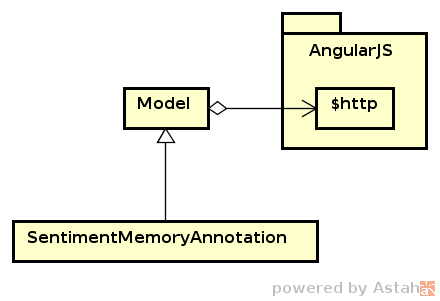
\includegraphics[height=4cm]{annotation_angular}
\caption{
Diagramma delle classi sul servizio \textit{AngularJS} sulle annotazioni
}
\label{fig:annotation_angular}
\end{center}
\end{figure}

\subsubsection{Test}
I test programmati con il tutor aziendale sono stati rivolti esclusivamente
sulle operazioni necessarie allo sviluppo dell'editor che consistevano:
aggiornamento dell'attributo \textit{status} di una annotazione e
ottenimento di tutti i valori assunti da \textit{category} in tutte le
annotazioni. I motivi sono spiegati nella prossima sezione.

Visto che si trattava di testare i metodi di un servizio la quale richiede un
\gls{back-end} si è ricorso all'uso di uno \gls{stub} per imitare le sue
risposte evitando d'introdurre i tempi di \textit{roundtrip} del sistema.
Lo \gls{stub} è stato creato usando il servizio \textit{\$httpBackend} di
\textit{AngularJS} con il quale è molto semplice configurare il risultato in
base alla richiesta.

\subsection{Interfaccia web}
\subsubsection{Requisiti}
Una volta create il servizio per accedere alle annotazioni è possibile produrre
l'interfaccia con la quale un \textbf{Senior Analyst} potrà scegliere quali far
entrare nel glossario.

L'interfaccia doveva visualizzare ogni annotazione con i relativi campi
informativi e, molto importante, doveva essere possibili mostrare le recensioni
in cui appariva. Quest'ultimo fattore era essenziale al moderatore per eseguire
operazioni di verifica sull'annotazione, in quanto, garantisce il contesto da
cui l'annotazione proviene. In caso di un'annotazione poco chiara, solo
attraverso il testo originale si sarebbe potuto valutarla e attuare una scelta o
di rifiuto o d'integrazione nel glossario.

Lo stato dell'annotazione doveva essere ben visibile e selezionabile tra i tre
stati possibili.

Il numero delle annotazione sarebbe potuto diventare molto grande quindi era
necessario raggruppare le annotazioni in gruppi e mostrarne solo uno per volta.
Se il \textbf{Senior Analyst}, attraverso un pulsante apposito, ne faceva
richiesta il successivo gruppo d'annotazioni sarebbe stato aggiunto a quelli già
presenti. Ogni gruppo doveva essere formato da dieci annotazioni, un numero per
l'azienda equilibrato che non imponeva costantemente di richiedere un successivo
gruppo e neanche affollasse lo schermo di annotazioni irrilevanti.

Infine, bisognava creare un filtro di ricerca in base alla categoria dell'
annotazione ed al suo stato. Oltre, per esempio, mostrare solo le nuove
annotazioni da revisionare, il \textbf{Senior Analyst} avrebbe potuto sottoporre
un glossario ad una serie di aggiunte e rimozioni tra annotazioni nuove,
integrate o precedentemente archiviate, cosi da migliorarne la qualità.

Il risultato doveva essere integrato con l'applicazione web dove vengono tenuti
tutti gli strumenti riguardanti le recensioni e, di conseguenze, le annotazioni.

\subsubsection{Sviluppo}
Il layout dell'applicazione è risultato minimalista dato il tempo a disposizione
per realizzarlo.

La pagina web è divisa in due parti: \textit{header} e \textit{tabella}.

L'\textit{header} è costituito dal titolo dell'applicazione, link di ritorno
alla pagina principale e sotto il filtro per le annotazioni. Soddisfacendo i
requisiti, il filtro è composto da due elementi: barra di ricerca per
selezionare la categoria e selettori dello stato dell'annotazione.

La barra di ricerca è un riutilizzo di quella sviluppata dalla Wonderflow, usata
in tutte le applicazioni in cui è richiesta cosi da garantire al fruitore
familiarità con lo strumento. La barra si presenta come un form di testo
tradizionale ma una volta preso il \textit{focus} mostrerà, attraverso una lista
a scorrimento, tutte le categorie in cui le annotazioni sono registrate. La
ricerca avviene tramite la digitazione di testo nell'area testuale, durante
il quale verranno tenuti tutti i possibili riscontri per lo spezzone scritto
mentre gli altri verranno eliminati dalla lista.

Per quanto riguarda il selettore dello stato la sua rappresentazione avviene
tramite tre radio button camuffati in tre bottoni allineati grazie all'uso
della libreria \textit{bootstrap}. Grazie ad essa oltre che un guadagno in
termini d'accessibilità lo è anche in estetica, risultando un buon colpo
d'occhio rispetto ai classici tre pallini selezionabili.

Entrambe queste componenti portano alla modifica della tabella a centro pagina
dove ogni riga rappresenta un'annotazione presente nell'archivio. La scelta
d'uso di una tabella è per poter visualizzare ogni attributo dell'annotazione
in modo chiaro, mantenendo un'alta leggibilità necessaria in caso di sessioni
prolungate di moderazione. La maggior parte degli attributi viene mostrato come
testo senza alcuna interazione, al contrario delle celle per il campo
\textit{reviews} e \textit{status}.

Nelle celle \textit{reviews} appare un numero indicante in quante recensioni
l'annotazione era stata individuata. Il numero è legato ad il \textit{link} per
la pagina di visualizzazione delle recensioni con sottolineato il testo dell'
annotazione interessata. In questo modo quando l'\textbf{analista} desidera
controllare l'origine dell'annotazione gli basta premere sul link per ottenere
tutte le recensioni in cui appare. Il formato di questa pagina segue la stessa
dell'editor testuale agevolando l'utente nella navigazione. L'unica differenza
sta nell'impossibilità di modificare o annotare le recensioni, limitando
l'interazione alla sola lettura. L'approccio scelto soddisfa il requisito ma
risulta inefficace per quanto concerne l'usabilità del sistema, imponendo
l'utente di consumare due ``\textit{click}'' del mouse per eseguire un'
operazione di rilievo, uno per saltare alla pagina delle recensioni ed uno per
tornare indietro. Tuttavia, dopo una discussione con il proponente, la mancata
visione di un'\textit{opportunity} generava un esiguo livello d'interesse ad un
cambio d'impostazione del layout, giungendo alla scelta di mantenere quello
realizzato.

Le celle \textit{status} invece contengono tre pulsanti con il quale si va sia a
visualizzare lo stato dell'annotazione e sia permettere al
\textbf{Senior Analyst} di cambiarglielo. I tre pulsanti vengono colorati di due
colori distinti: blu lo stato attivo e grigio gli altri; permettendo con
semplicità comprendere in quale stato l'annotazione si trovi. Essendo pulsanti,
basta premere su quello che rappresenta lo stato voluto per inviare la richiesta
di aggiornamento (le operazioni sono svolte nel \gls{front-end} ma i dati sono
nel \gls{back-end}). Se l'operazione avviene senza errori allora il pulsante
appena premuto si colorerà di blu e l'altro diverrà grigio, altrimenti apparirà
sullo schermo un messaggio d'errore.

Il cambio di stato dell'annotazione è una delle possibili azioni vincolate alla
comunicazione con il \textit{back-end} via \textit{Internet} e la lettura e
scrittura dei dati nel \textit{database}; quindi affette da possibili errori.
La gestione è stata affrontata in linea a quanto accade nelle altre
applicazioni ovvero attraverso l'\textit{alert}, scrivendo la causa dell'errore
e la richiesta di contattare il responsabile tecnico per segnalarvi il
malfunzionamento.

\subsubsection{Test}
L'applicazione web è stata il primo punto di prova degli \gls{E2ET} utilizzando
la libreria \textit{Protractor}. Come discusso nella sezione
\nameref{sec:tecnologie} la libreria è studiata per integrarsi nell'ambiente
\textit{AngularJS}, aggiungendo al ricco \textit{set} di strumenti l'esecuzione
dei test in un \textit{browser} reale dov'è possibile, attraverso le \gls{API}
di \textit{Protractor}, simulare ogni aspetto dell'applicazione e controllare
lo stato di ogni elemento nell'interfaccia. Attraverso di essa, effettuare una
verifica sulla cooperazione degli elementi che compongono l'interfaccia diventa
semplice ed elegante.

La metodologia utilizzata alla Wonderflow è la creazione preventiva di un
oggetto utente in cui eseguire le operazioni salienti dell'applicazione. L'uso
di un utente virtuale conferisce un mezzo con cui veicolare il test, mantenendo
un altissimo livello d'astrazione completamente indipendente dalla
progettazione del sistema. Anche dopo uno stravolgimento dell'architettura di
base se il risultato rimane invariato, essendo gli \gls{E2ET} \textit{black box}
di natura, non sarò necessario alcun intervento d'aggiornamento sul codice
dei test. L'oggetto utente avrà come metodi tutte le operazioni che il fruitore
dell'applicazione naturalmente svolge. Contare il numero di righe di una
tabella o leggere del testo o guardare il colore di un elemento della pagina
sono tutti esempi di possibili azioni che vanno tradotte in metodi dell'oggetto.

In specifico al moderatore delle annotazioni è stato realizzato un test per
ognuno dei seguenti casi d'uso:
\begin{itemize}
\item Visualizzazione delle annotazioni (UC1 - \ref{fig:uc_1})
\item Filtro per categoria (UC2 - \ref{fig:uc_2}) e stato (UC3 - \ref{fig:uc_3})
\item Richiesta del successivo gruppo d'annotazioni (UC4 - \ref{fig:uc_4})
\item Visualizzazione recensioni associate alle annotazioni (UC5 -
\ref{fig:uc_5})
\end{itemize}

Non tutti i test erano verificabili immediatamente dopo il caricamento della
pagina web, alcuni richiedevano una serie di passaggi per portare alla
visualizzazione del risultato interessato. Come detto ogni azione corrisponde
ad un metodo nell'oggetto utente e ogni metodo è realizzato con le sapienti
\gls{API} di \textit{Protractor}, risultando una continua generazione di
\textit{Promise} ad ogni invocazione. Grazie alla loro proprietà di
``incatenamento'' si è in grado di pilotare l'utente virtuale realizzando una
serie di compiti da fargli svolgere, portando al completamento del compito.

La progettazione dell'utente non era banale. Il rischio di produrre azioni
troppo complesse, non sfruttando la concatenazione delle azioni, e troppo
specifiche sull'applicazione da testare, non sfruttando la loro generalità,
era presente, vista l'unicità dell'entità da rappresentare. C'era anche da
considera il rovescio della medaglia. Azioni troppo generiche o troppo piccole
avrebbero portato ad una sicura verbosità ed una notevole lunghezza della catena
di compiti da eseguire. Il risultato è mostrato in figura \ref{fig:user_test}.

\begin{figure}[H]
\begin{center}
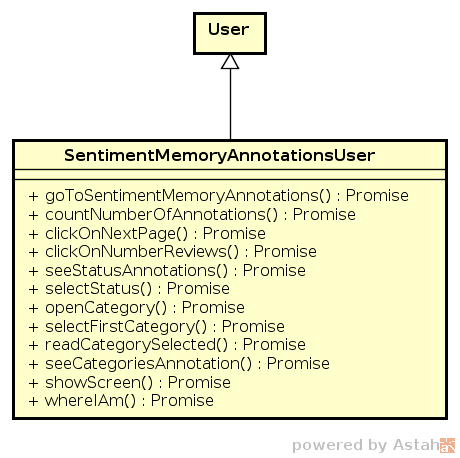
\includegraphics[height=7cm]{user_test}
\caption{
Diagramma delle classi sull'utente virtuale per la moderazione del glossario
}
\label{fig:user_test}
\end{center}
\end{figure}

\begin{center}
\begin{lstlisting}[
  frame=single,
  caption=Codice test per UC4,
  label=code:uc_4,
  language=Java
]
describe('USE CASE: get other annotations', function () {
  it(
    'when user clicks "More terms" the other annotations appear',
    function () {
      return user.clickOnNextPage().then(function () {
        return user.countNumberOfAnnotations();
        /**
         * Si effettua il concatenamento. Il risultato della
         * Promise precedente diventa il parametro di quella
         * successiva.
         */
      }).then(function (count) {
        expect(count).toBeGreaterThan(10);
      });
    });
  }
);
\end{lstlisting}
\end{center}

Come si può vedere i nomi dei metodi equivalgono alla descrizione dell'azione
da compiere. Si è pensato di dividere di creare una gerarchia d'utenti in modo
da inserire azioni generiche nella classe base (vai in una pagina, login, ecc...
) e le azioni più specifiche dell'applicazione nella classe derivata (conta
annotazioni, clicca sul numero di recensioni, ecc...). Ora i test per i casi
d'uso non è altro che la disposizione in modo ordinato delle possibili azioni
con l'inserimento di un \textit{oracolo} a risultato compiuto. Il gruppo d'
immagini \ref{fig:uc_user} mostra per ogni attività il relativo metodo da
invocare, concludendo con la verifica eseguita dall'oracolo.

Per completezza mostro il frammento di codice che esegue il test per il caso d'
uso UC4, snippet \ref{code:uc_4}. Come si può notare l'oggetto ``\textit{user}''
esegue i suoi metodi man mano che si scende nella catena delle \textit{Promise}.
La catena viene realizzata tramite il \textit{.then()} la quale prende in input
il valore restituito dalla risoluzione della \textit{Promise} precedente,
oppure, se il risultato fosse un'ulteriore \textit{Promise} verrebbe prima
risolata e dopo il risultato verrebbe passato a quella successiva.

\begin{figure}[H]
\centering
\subfigure[Diagramma di sequenza caso d'uso UC1]{
  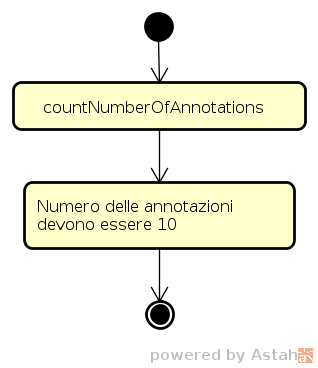
\includegraphics[width=.25\linewidth]{uc_1}
  \label{fig:uc_1}
}
\hfill
\subfigure[Diagramma di sequenza caso d'uso UC3]{
    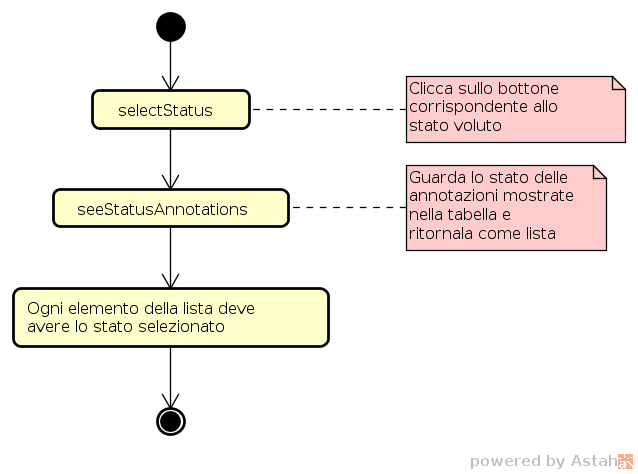
\includegraphics[width=.45\linewidth]{uc_3}
    \label{fig:uc_3}
}
\hfill
\subfigure[Diagramma di sequenza caso d'uso UC4]{
    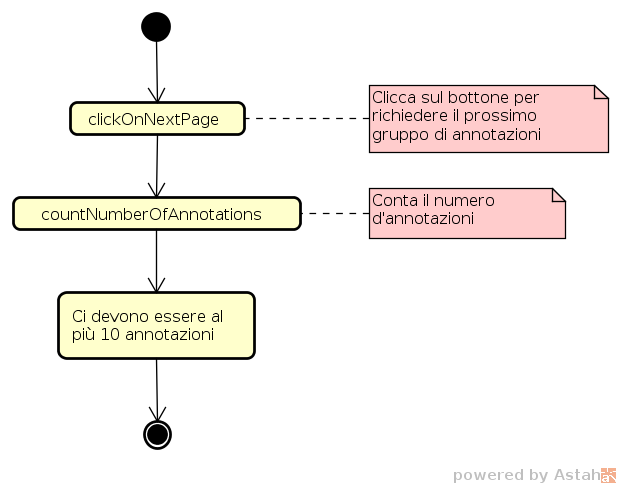
\includegraphics[width=.4\linewidth]{uc_4}
    \label{fig:uc_4}
}
\hfill
\subfigure[Diagramma di sequenza caso d'uso UC5]{
    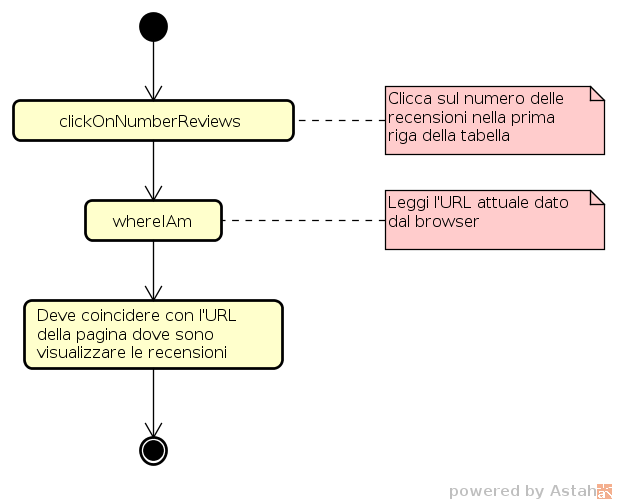
\includegraphics[width=.4\linewidth]{uc_5}
    \label{fig:uc_5}
}
\hfill
\subfigure[Diagramma di sequenza caso d'uso UC2]{
    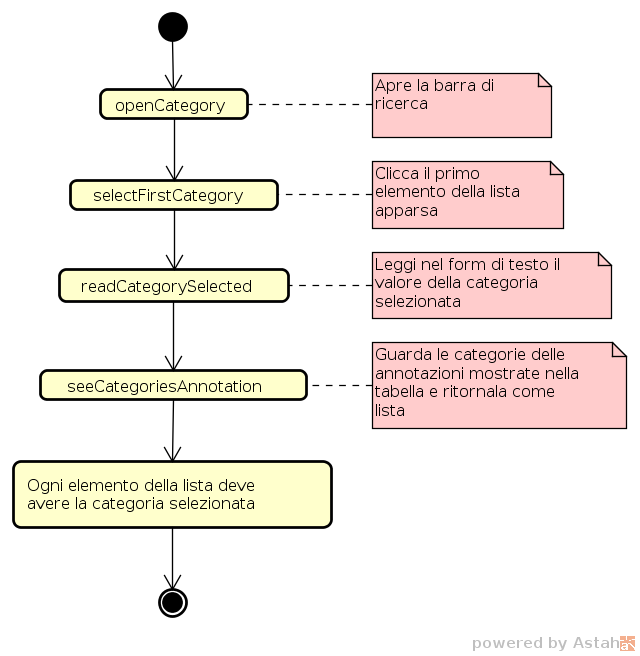
\includegraphics[width=.4\linewidth]{uc_2}
    \label{fig:uc_2}
}
\caption{Diagranna di sequenze per i casi d'uso}
\label{fig:uc_user}
\end{figure}

\newpage

\section{Refactoring del BaaS}
\subsection{Stato iniziale}
Una mansione da svolgere era pulire dallo stesso \gls{BaaS} utilizzato dall'
applicazione web alcune smagliature lasciate durante le fasi di sviluppo.

Il \gls{BaaS} si presenta come l'unione di quattro pacchetti \textit{npm}:
\begin{itemize}
\item restful-mongo-utils
\item restful-mongo2
\item wonderflow-api-app2
\item admin.api.wonderflow.co
\end{itemize}
ognuno progettato per svolgere un compito diverso come la \textit{Filosofia
Unix} suggerisce. Si parlerà di ogni componente nelle sezioni successive.

Tuttavia, questa gestione di profonda modularizzazione del codice e le norme d'
uso del \textit{CVS} ha favorito un'approccio errato nello sviluppo del codice.
L'errore commesso infatti è strettamente legato a come \textit{npm} gestisce le
dipendenze di un pacchetto, quindi è necessario avere un quadro generale del
meccanismo.

In breve, ogni dipendenza dichiarata nel \textit{package.json} viene installata
all'interno di una cartella generata da \textit{npm} stesso chiamata
\textit{node\_modules}. Dentro alla directory sono presenti tante directory
quante sono le dipendenze e al loro interno si trovano i loro file sorgenti e
un'ulteriore cartella \textit{node\_modules} in cui sono installati le
dipendenze. L'iterazione di cartelle \textit{node\_modules} continua finché non
si installi una sottodipendenza che non ha alcun legame con altri pacchetti.
Vista nel suo complesso, l'installazione delle dipendenze forma un albero che ha
come radice il progetto corrente e come nodi le varie dipendenze.

Ora inseriamo la variabile versione al sistema delle dipendenze. Nel
\textit{package.json} è possibile definire la versione delle dipendenze
attraverso vari operatori che conferisco elasticità o rigidità all'insieme di
scelte delle versioni. Facendo un esempio, nella dichiarazione della dipendenza
ad un pacchetto ``A'' si può scegliere fra i seguenti operati:
\begin{itemize}
  \item > o < la dipendenza deve avere una versione almeno maggiore o più bassa
  del valore specificato
  \item \~{} o = indicano d'installare la version più vicina o esatta di quella
  specificata
\end{itemize}
cosi l'autore di un pacchetto dovrebbero avere il pieno controllo delle
dipendenze che verranno installate, garantendogli la stabilità del codice che è
fondamentale quando si mette in pubblica un servizio come il \gls{BaaS}.
Sorprendentemente però la situazione non è cosi. La scela della versione delle
dipendeze è limitata a solo il primo livello dell'albero, lasciando per i
livelli successivi quelle specificate dall'autore. Perciò non è possibile
garantire che l'istanza dell'albero delle dipendenze rimanga costante.
Poniamo nell'esempio che ``A'' abbia come dipendenza ``B''. Se l'autore di ``A''
avesse specificato che la versione ``B'' potesse essere una qualunque superiore
ad una soglia minima, ciò implicava che nel momento in cui vi fossero nuove
versioni di ``B'' queste verrebbero installate. Dunque se al primo livello
fissassi la versione di ``A'' non ci sarebbe alcuna garanzia di ottenere sempre
la stessa versione di ``B'', portando ad un'instabilità di fondo nel sistema.
La Wonderflow decise di risolvere il problema inserendo nei \textit{repository}
Git lo stato della directory \textit{node\_modules} nel momento in cui il
software risultasse maturo da essere rilasciato. Cosi facendo ogni installazione
del software avrebbe mantenuto versioni consistenti delle dipendenze, garantendo
stabilità.

Tuttavia l'approccio scelto viola un principio del software del controllo di
versione, ossia: non effettuare il \gls{check} dei file derivati direttamente da
altri tramite una semplice trasformazione. In questo caso la trasformazione è
l'installazione delle dipendenze effettuata da \textit{npm}, partendo dal file
\textit{package.json}, sfociando in una \textit{ridondanza} dei dati e portando
il controllo di versione ad essere \textit{error-prone}\footnote{Propenso all'
errore}.

La situazione riguardante i quattro pacchetti \textit{npm} era la seguente: ad
ognuno era associato un repository \textit{Git} dove effettuare il controllo di
versione. Per il discorso sulla stabilità del software, all'interno dei
repository erano presenti anche i rispettivi \textit{node\_modules} con le
dipendenze installate. Ora, la relazione tra i pacchetti era d'incapsulamento
l'uno di seguito all'altro fino ad arrivare ad \textit{admin.api.wonderflow.co};
colui che completa ed avvia il \gls{BaaS}. Ciò comporta che anche le dipendenze
sono innestate l'una dentro l'altra e, per via del limitato controllo, solo
nella dipendenza figlia si ha un controllo diretto.

Nello scenario di una modifica di uno dei moduli, affinché si aggiornino
tutti, sarebbe necessario applicare la procedura d'installazione ricorsivamete
nei repository dei moduli salendo i livelli di dipendenza fino ad arrivare ad
\textit{admin.api.wonderflow.co}, la radice dell'albero; con la conseguente
perdita cospicua di tempo.

A causa di tempistiche strette, lo sviluppo e gli aggiornamenti delle dipendenze
vennero effettuati nelle versioni all'interno di \textit{node\_modules} in
\textit{admin.api.wonderflow.co}, evitando di eseguire i passaggi d'
aggiornamento ma lasciando versioni obsolete del codice nei \textit{repository}.

Il principale compito da svolgere era riportare il codice sorgente nei propri
\textit{repository}, rimpiazzando il codice con quello aggiornato in modo da
tornare allo sviluppo separato delle componenti. Durante lo spostamento ci si è
anche impegnati a risolvere alcune magagne progettuali, tentando di scongiurare
possibili malfunzionamenti futuri. In ogni sezione si spiegheranno i problemi
riscontrati e le soluzioni adottate.

\subsection{Ristrutturazione HTTP Handler}
\subsubsection{Requisiti}
Il pacchetto \textit{restful-mongo-utils} ha il compito di esportare gestori per
le richiesta HTTP \textit{get, post, put} e \textit{delete}. I gestori vengono
realizzati tramite funzioni in cui andavano a implementare la logica per l'
accesso ai dati nei \textit{database MongoDB}, fornendo cosi le \gls{API}
generiche utilizzate per sopperire il bisogno di costruire un \gls{back-end}
``ad hoc'' per le applicazioni web.

Nella situazione precedente al \gls{refactoring} i gestori esposti coprivano
solo le richieste \textit{put e delete}, mente per \textit{get} e \textit{post}
erano stati sviluppati direttamente nel pacchetto \textit{restful-mongo2} il
quale ambisce a tutt'altro scopo. In più l'organizzazione interna di
\textit{restful-mongo-utils} era spartana, inadatta alle possibili evoluzioni
del software. In figura \ref{fig:restful_mongo} è rappresentata la situazione
originale.

Svolgere degli interventi per spostare i gestori HTTP dal pacchetto
\textit{restful-mongo2} e riorganizzare \textit{restful-mongo-utils} avrebbe
di sicuro giovato al sistema complessivo.

\begin{figure}[H]
\begin{center}
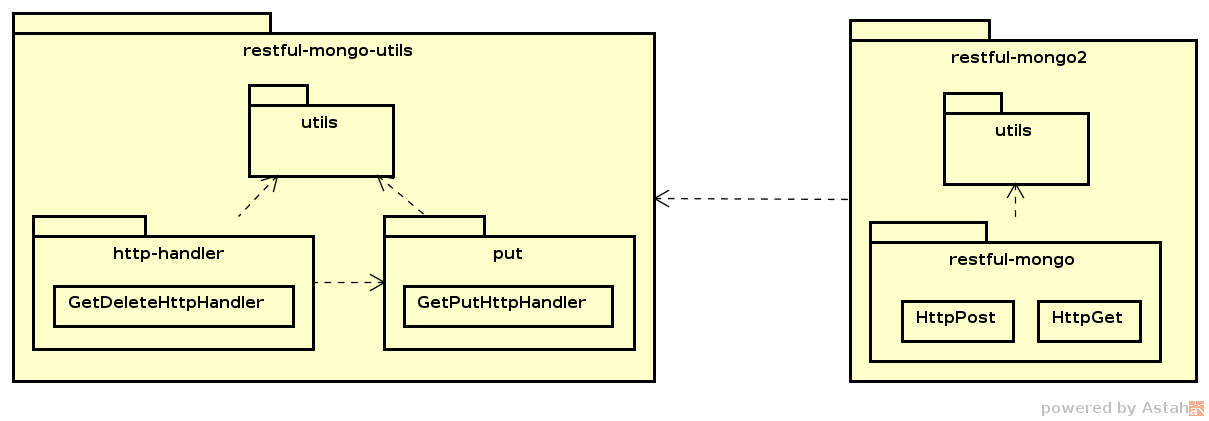
\includegraphics[height=5cm]{restful_mongo}
\caption{
Diagramma delle classi sulla composizione degli \textit{HTTP Handler}
}
\label{fig:restful_mongo}
\end{center}
\end{figure}

\subsubsection{Sviluppo}
La prima operazione compiuta è stata portare ``\textit{HttpGet}'' e
``\textit{HttpPost}'' in \textit{restful-mongo-utils}. Inoltre il package
``\textit{restful-mongo2::utils}'' è stato integrato con
``\textit{restful-mongo-utils::utils}'' in quanto possedeva alcuni strumenti
usati per i gestori dei metodi \textit{get} e \textit{post}. Una volta
raggruppati tutti gli \textit{handlers} HTTP si è ristrutturato il pacchetto
come mostrato in figura sotto (\ref{fig:ref_restfulmongo}).

\begin{figure}[H]
\begin{center}
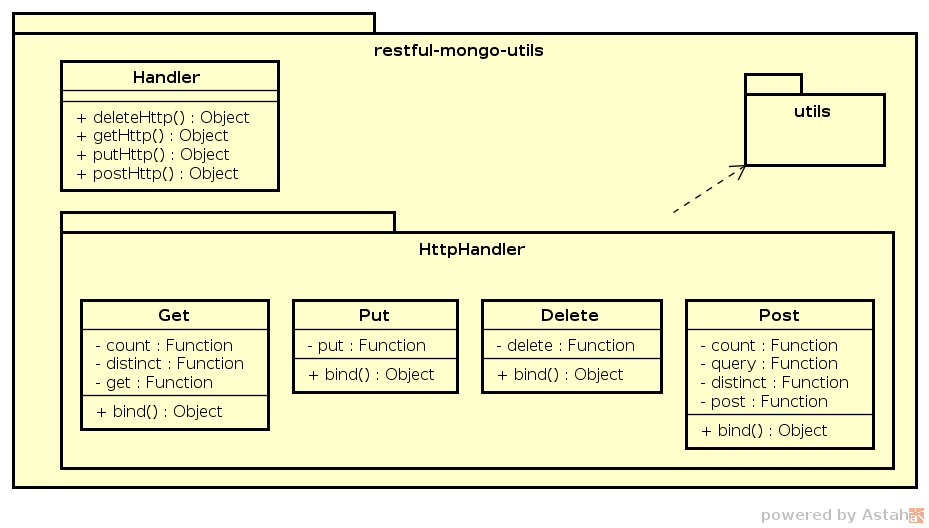
\includegraphics[height=7cm]{ref_restfulmongo}
\caption{
Diagramma delle classi \textit{restful-mongo-utils} dopo il \textit{refactoring}
}
\label{fig:ref_restfulmongo}
\end{center}
\end{figure}

I gestori ora sono stati convertiti in classi dove ogni attributo è un funtore
associato ad un \gls{API}, risultando una struttura più pulita. Il metodo
\textit{.bind()} ha lo scopo di poter esportare i funtori al di fuori dalle
classi ma mantenendo il riferimento al giusto \textbf{this}. Nelle applicazioni
\textit{Express}, dove le risorse corrispondono a delle \textit{callback},
diventava impossibile utilizzare \textit{restful-mongo-utils} senza questo
approccio. Ovviamente diventava necessario invocare sempre il \textit{.bind()}
prima di utilizzare i funtori ed è per questo che ``\textit{Handler}'' è stata
inserito. La classe implementa il \textit{Façade pattern}, dando un unico punto
d'accesso al pacchetto, e fornisce i funtori esportati correttamente invocando
il metodo \textit{.bind()}. Un'obiettivo raggiunto dal \textit{Façade} era l'
esposizione di un'interfaccia compatibile a quella della versione prima.
In tal modo non sarebbe stata necessario alcuna operazione d'adattamento in
\textit{restful-mongo2}, velocizzando il completamento del \textit{refactoring}.

\subsubsection{Test}
I test svolti sono stati importati sia dalla vecchia versione di
\textit{restful-mongo-utils} e sia da \textit{restful-mongo2}, nel quale
andavano a verificare il funzionamento dei funtori dei gestori e la loro
corretta integrazione con un'applicazione \textit{Express}. Il riutilizzo dei
test è stato pensato per poter accertare la completa retrocompatibilità con
l'interfaccia precedente.

\subsection{Ristrutturazione applicazione Express}
I tre pacchetti mancanti da ristrutturare condividono il medesimo obiettivo:
provvedere \gls{API} all'applicazione \textit{Express}.

Infatti ognuno di loro prendevano un oggetto \textit{Express} dove definire per
ogni metodo HTTP un \gls{API} legata ad un certo ambito, nello specifico:
\begin{itemize}
\item \textit{restful-mongo2} - operazioni \textit{CRUD} al database
\item \textit{wonderflow-api-app2} - gestione utenti e privilegi d'accesso
\item \textit{admin.api.wonderflow.co} - sezione amministratore e avvio
\gls{back-end}
\end{itemize}

tutte insieme fornivano le funzionalità richieste dal sistema \gls{BaaS}.

Nell'ottica del \textit{refactoring} ad ognuna di loro è stata applicata la
medesima procedura: installazione della dipendenza aggiornata, sostituzione del
codice nel proprio \textit{repository} ed esecuzione dei test d'unità, senza
alcun ulteriore intervento.

\subsection{Collaudo e pubblicazione}
Una volta conclusa l'operazione di \textit{refactoring} era possibile passare
a testare che le modifiche apportate non abbiano introdotto errori per il quale
le applicazioni web generavano comportamenti anomali. La Wonderflow archivia
tutta una batteria di \gls{E2ET} dove vanno a simulare ogni azione di rilievo
delle varie applicazioni web, la quale richiedono il \gls{BaaS} per funzionare.
L'ambiente di simulazione d'interazione tra \gls{front-end} e \gls{back-end}
veniva costruito sfruttando l'eccezionale sistema di composizione offerto da
\textit{Docker}. Praticamente si creano tre \textit{immagini Docker}, una per
ognuna delle parti coinvolte, e si va a comporre l'infrastruttura del sistema
da modellare. Le immagini rappresentano il componente autonomo del sistema, con
tutte le risorse necessarie per eseguire. Nel caso del \gls{BaaS} ristrutturato,
l'immagine conterrà il pacchetto \textit{admin.api.wonderflow.co}, tutte le
sue dipendenze nel \textit{node\_modules} e un file di configurazione con
descritta la procedura d'avvio dell'applicazione \textit{Express} una volta
che l'immagine sarà montata. Le immagini eseguite da \textit{Docker} vengono
chiamate \textit{container}.

Il sistema di test (immagine \ref{fig:stack_docker}) sarà in esecuzione al
fianco del sistema operativo e sarà perciò interagibile in ogni istanze.

Quando il \gls{BaaS} avrà superato tutti gli \gls{E2ET} sarà possibile
pubblicare la nuova versione dell'immagine \textit{Docker} ed installarla nei
server aziendali.

\begin{figure}[H]
\begin{center}
\includegraphics[height=7cm]{stack_docker}
\caption{
Rappresentazione dell'infrastruttura composta tramite \textit{Docker}
}
\label{fig:stack_docker}
\end{center}
\end{figure}

\section{Generatore Yeoman per applicazioni AngularJS}
\subsection{Requisiti}
\textit{AngularJS} spinge alla divisione in componenti e al loro massiccio
riutilizzo. Tuttavia l'inizio di un loro sviluppo diventava una procedura
macchinosa e ripetitiva: tra inizializzazione del pacchetto \textit{npm},
quello \textit{Bower.js}\footnote{molto simile ad \textit{npm} ma orientato per
il web} e le configurazione di \textit{karma}, lo sviluppatore doveva spendere
 vari minuti per ottenere un ambiente di lavoro operativo.

La Wonderflow ha pensato che un miglioramento nello sviluppo sarebbe stato di
rimuovere il tempo di \textit{overhead} per costruire componenti
\textit{Angular.js} attraverso un \textit{Yeoman Generator}.

\textit{Yeoman} è programma, sempre nell'ambiente \textit{Node.js}, il quale
gestisce generatori script previsti per la creare strutture come file o
directory. I generatori sono pacchetti \textit{npm} che seguono la struttura
imposta da \textit{Yeoman} che, brevemente, richiede di inserire il progetto
in una cartella nominata ``generators'' e, da li in poi, ogni sottocartella
definisce le parti del progetto realizzabili.

Il generatore doveva poter essere in grado di creare:
\begin{itemize}
\item direttive \textit{Angular.js}, con relativi test
\item servizi \textit{Angular.js}, con relativi test
\item ambiente di lavoro con configurazione di \textit{npm}, \textit{bower} e
\textit{karma}
\end{itemize}

Inoltre alcuni aspetti richiedevano la configurazione manuale perciò era
importante utilizzare i sistemi d'interazione offerti da \textit{Yeoman} per
permettere all'utente di scegliere alcune opzioni

\subsection{Sviluppo}
Essendo tre le parti generabili da \textit{Yeoman}, all'interno della cartella
``generator'' sono stati inserite le sottocartella: \textit{app},
\textit{service} e \textit{directive}; ognuna tiene la logica di costruzione
delle varie parti del progetto ed i template dei file che verranno creati.
\textit{Yeoman} elabora i template utilizzando \textit{EJS}, una libreria
leggera e performante nella quale attraverso un sistema di segnaposti e
\textit{scope} simile ad \textit{AngularJS} divide molto bene il contenuto,
generato dalla logica, dalla presentazione, il contenuto statico del file.

Nei seguenti paragrafi sono trattati i componenti descrivendone la struttura e
la creazione.

\paragraph{app}
Soddisfa l'inizializzazione dell'ambiente di sviluppo, generando la struttura
dei file seguenti:
\begin{center}
\begin{lstlisting}[
  frame=single,
  caption=Struttura progetto inizializzato
]
\
+ npm.json
+ bower.json
+ karma.conf.js
\end{lstlisting}
\end{center}

Tramite i primi il componente \textit{AngularJS} ha già le dipendenze dichiarate
ed alcuni campi informativi riempiti con i valori di base. Il file
``\textit{karma.conf.js}'' dichiara l'ambiente con il quale eseguire gli
\gls{E2ET} del componente, al cui interno sono già definite le opzioni usate
comunemente dall'azienda.

I parametri richiesti dall'utente riguardano il nome del componente, una sua
descrizione e la licenza con il quale pubblicarlo. Tutte sono inseribili all'
avvio del generatore tramite l'interfaccia da terminale offerta da
\textit{Yeoman}.

\paragraph{service}
Soddisfa la crezione di un servizio \textit{AngularJS} con l'inserimento del
relativo file di test. La struttura generata era la seguente:
\begin{center}
\begin{lstlisting}[
  frame=single,
  caption=Struttura servizio \textit{AngularJS}
]
\
+ `name`.js
+ test/
+ --- spec/
+ --- --- `name`.js
\end{lstlisting}
\end{center}

Il generatore crea il servizio già con l'intestazione pronta, lasciando allo
sviluppatore solo la programmazione del corpo centrale. Il nome del file sono
tra apici perché indicano che il nome del servizio è un parametro preso in
input all'avvio del generatore. In questo caso, il generatore esegue il
\textit{parsing} delle opzioni dalla linea di comando data per avviarlo.

\paragraph{directive}
Soddisfa la creazione delle direttive \textit{AngularJS}. La struttura generata
era identica a quella per il \textit{service}, con l'unica differenze
riscontrabile nel contenuto dei file. In ogni caso, anche qui lo sviluppatore si
troverà i file con l'intestazione pronta, necessitando solo la realizzazione
della direttiva.

\subsection{Test}
La particolarità di produrre test per generatori \textit{Yeoman} sono due:
creazione di un ambiente temporaneo di test e formazione di \textit{driver} per
il passaggio delle opzioni. La prima è per verificare che le condizioni dello
scenario di lavoro soddisfi i requisiti. La seconda invece è per controllare il
comportamento del generatore in base all'input. Per entrambe \textit{Yeoman}
offre due librerie specifiche per raggiungere l'obiettivo.
